\documentclass[../report.tex]{subfiles}
\begin{document}

\chapter{Interprete}\label{c:interprete}
\section{Bytecode}\label{s:bytecode}
Il bytecode generato dal metodo \verb|String codeGeneration()| dei nodi dell'AST rispetta le regole della grammatica descritta nel file \verb|svm/lexer/SVM.g4|. Il linguaggio si ispira al set d'istruzioni Assembly x86. 
\begin{figure}[H]
    \centering
    
\includegraphics[width=0.9\textwidth]{istruzioneCodiceGenerato}
    \caption{Schema istruzioni codice generato.}
    \label{fig:istruzione-codice-generato}
\end{figure}
Un'istruzione \`e composta da diverse componenti, alcune obbligatorie, altre invece, opzionali:
\begin{itemize}
    \item \textbf{Istruzione}: stringa che permette di differenziare le diverse istruzioni. \`E l'unica componente obbligatoria in ogni istruzione e, nel caso di un'etichetta \`e utilizzata per dare il nome all'etichetta che si sta definendo;
    \item \textbf{Primo argomento}: stringa opzionale che permette in alcune istruzioni di specificare un registro o un'etichetta;
    \item \textbf{Offset}: numero opzionale che permette di specificare quanto sommare al valore contenuto nel secondo argomento;
    \item \textbf{Secondo argomento}: stringa opzionale che permette in alcune istruzioni di specificare un registro o un numero;
    \item \textbf{Terzo argomento}: stringa opzionale che permette in alcune istruzioni di specificare un registro, un numero o un'etichetta;
\end{itemize}
Per ogni istruzione letta, viene creato un oggetto di tipo \verb|SVMInstruction| la cui classe \`e definita in \verb|svm/instruction/SVMInstruction.java|.
\section{CPU e memoria}\label{s:cpu-e-memoria}
L'interprete emula il comportamento di una CPU e di una memoria.
\subsection{CPU}
La CPU esegue le istruzioni passate al costruttore dell'interprete. Il metodo \verb|run| esegue un ciclo finch\'e o la memoria non ha pi\`u celle a disposizione o si raggiunge l'istruzione \verb|halt|. A ogni iterazione si accede all'istruzione indicata dal registro \verb|$ip| che viene poi incrementato di uno per l'iterazione successiva. Il comportamento da seguire dipende dall'istruzione, in particolare dal campo dati \verb|instruction| degli oggetti \verb|SVMInstruction|.

\subsection{Registri}
La CPU ha accesso a 8 registri:
\begin{itemize}
    \item \textbf{Instruction pointer} (\$ip): indica quale istruzione sar\`a la prossima a essere eseguita;
    \item \textbf{Stack pointer} (\$sp): punta alla cima dello stack;
    \item \textbf{Heap pointer} (\$hp): punta alla prima posizione libera dello heap;
    \item \textbf{Frame pointer} (\$fp): punta all'access link corrente relativo al frame attivo;
    \item \textbf{Access link} (\$al): registro utilizzato per attraversare la catena statica degli scope;
    \item \textbf{Return address} (\$ra): registro utilizzato per salvare l'indirizzo (numero d'istruzione) al quale ritornare una volta usciti da un frame;
    \item \textbf{Accumulatore} (\$a0): registro utilizzato per salvare il valore computato da alcune espressioni;
    \item \textbf{Registro general purpose} (\$t1): registro generico utilizzabile liberamente all'interno del codice generato.
\end{itemize}
Sono state scritte due funzioni per gestire i registri:
\begin{itemize}
    \item \verb|void updateRegister(String register, int value)| che aggiorna il contenuto del registro passato \verb|register| con il valore \verb|value|;
    \item \verb|int readRegister(String register)| che ritorna il valore contenuto nel registro \verb|register|.
\end{itemize}

\subsection{Memoria}
La memoria \`e gestita come un array di \verb|MemoryCell| diviso, logicamente, in due parti: lo stack e lo heap. Lo stack si sviluppa dalle ultime posizioni dell'array e ``cresce'' verso indici pi\`u piccoli mentre lo heap comincia a indice 0 e si sviluppa verso indici pi\`u grandi. Sono state scritte quattro funzioni per gestire la memoria:
\begin{itemize}
    \item \verb|void writeOnMemory(int address, int data)| che prende in input due interi: il primo \`e l'indice al quale andare a scrivere e il secondo \`e il dato da scrivere;
    \item \verb|void resetCell(int address)| che resetta, mettendo a \verb|null| il contenuto di una cella, questa funzione \`e comoda in quanto semplifica la visualizzazione della memoria durante il debug ma non sarebbe altrimenti necessaria;
    \item \verb|int readFromMemory(int address)| che ritorna il contenuto della memoria all'indirizzo passato in input;
    \item \verb|void freeMemory(int address)| che segna come ``libera'' una cella di memoria, viene chiamata alla \verb|delete| di un puntatore.
\end{itemize}

\subsubsection{MemoryCell}

\section{Record di attivazione}\label{s:record-di-attivazione}
Nella memoria, lo \textit{stack} \`e diviso in record di attivazione o \textit{frame}. Quando viene creato un nuovo \textit{scope} e quindi: nel main, all'invocazione di una funzione e in un nuovo blocco, viene fatto il \textbf{push} di un nuovo \textit{frame} e, quando si esce dallo \textit{scope}, ne viene fatto il \textbf{pop}.
\begin{figure}[H]
    \centering
    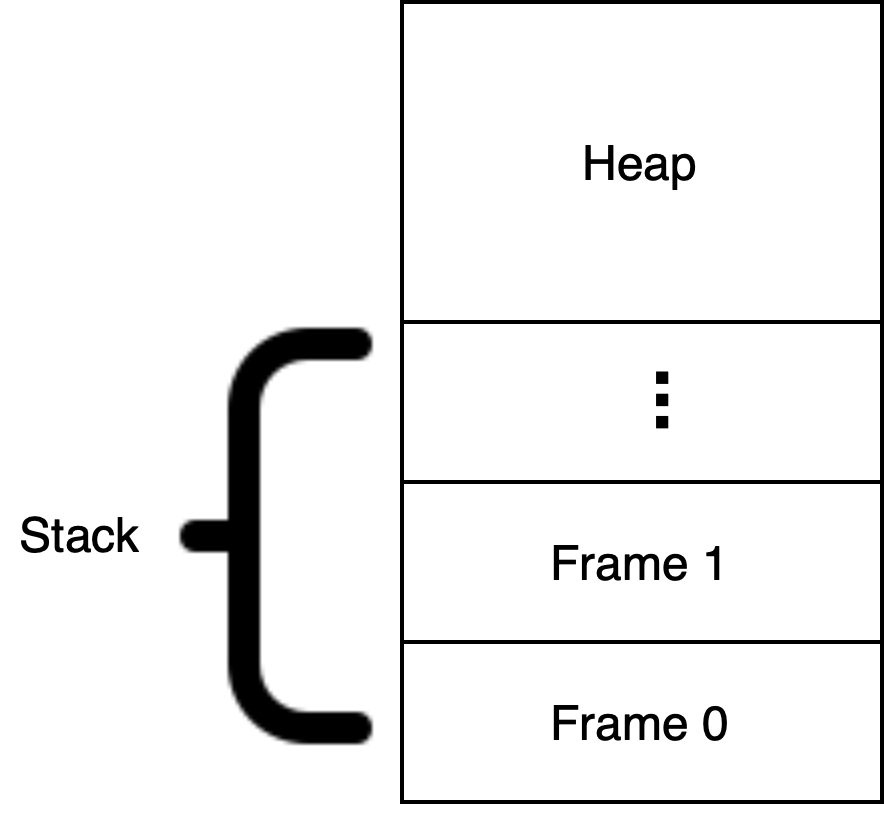
\includegraphics[width=0.5\textwidth]{organizzazioneMemoria}
    \caption{Memoria nell'interprete.}
\end{figure}
Ogni record di attivazione \`e composto sempre nello stesso modo:
\begin{figure}[H]
    \centering
    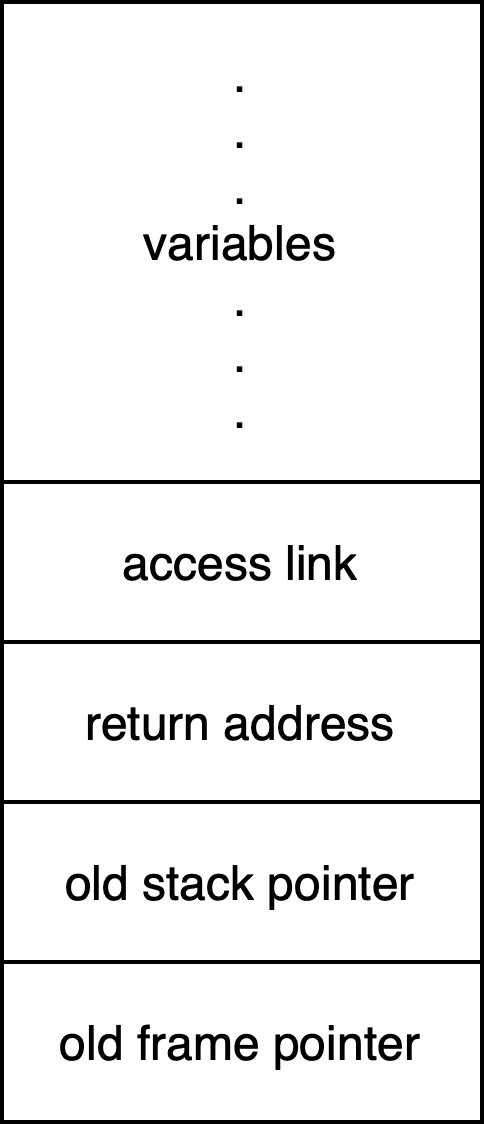
\includegraphics[width=0.3\textwidth]{organizzazioneFrame}
    \caption{Organizzazione di un record di attivazione.}
\end{figure}
\begin{itemize}
    \item \textbf{Old frame pointer}: utilizzato per memorizzare l'indirizzo del frame pointer precedente al push del nuovo \textit{frame};
    \item \textbf{Old stack pointer}: utilizzato per memorizzare l'indirizzo dello stack pointer precedente al push del nuovo \textit{frame};
    \item \textbf{Return address}: utilizzato per memorizzare il valore dell'instruction pointer cos\`i da sapere dove ritornare una volta terminata l'esecuzione di una funzione;
    \item \textbf{Access link}: utilizzato per risalire la catena statica degli \textit{scope} per accedere alle variabili dichiarate al di fuori del \textit{frame} corrente;
    \item \textbf{Variables}: spazio di memoria riservato alle variabili dichiarate all'interno dello \textit{scope} che il \textit{frame} rappresenta. Nel caso di chiamata di funzione, vengono prima messe le variabili passate come argomento e poi le variabili dichiarate nel blocco della funzione.
\end{itemize}

\section{Funzionamento dell'interprete}\label{s:funzionamento-interprete}
\subsection{Campi dati}
L'interprete e il suo funzionamento sono definiti all'interno della classe \verb|SVMInterpreter|. I suoi campi dati pi\`u rilevanti, in quanto necessari al corretto funzionamento, sono:
\begin{itemize}
    \item \textbf{code}: una lista di \verb|SVMInstruction|, generata dal parsing del codice generato, contiene la sequenza ordinata di istruzioni che l'interprete dovr\`a eseguire;
    \item \textbf{memorySize}: la dimensione massima che la memoria pu\`o raggiungere;
    \item \textbf{memory}: un vettore di \verb|MemoryCell|, rappresenta la memoria dell'interprete. Pu\`o essere logicamente divisa in due parti: lo \textit{heap} e lo \textit{stack}. Lo \textit{heap} cresce a partire dagli indici minori ($0, 1, 2, \dots$), mentre lo \textit{stack} cresce a partire dagli indici maggiori ($memorySize, memorySize - 1, memorySize - 2, \dots$);
    \item \textbf{registers}: una mappa che associa ad una stringa un intero. Le stringhe indicano i registri e, gli interi, il valore che quel registro assume;
    \item \textbf{\$ip}: registro speciale che indica quale istruzione si sta eseguendo. 
\end{itemize} 
Sono poi presenti altri campi dati utilizzati per semplificare il processo di debug e visualizzazione dello stato dell'interprete:
\begin{itemize}
    \item \textbf{lastUpdatedRegister}: indica l'ultimo registro aggiornato;
    \item \textbf{lastUpdatedMemoryCell}: indica l'indirizzo (l'indice del vettore \textit{memory}) di memoria aggiornato per ultimo;
    \item \textbf{globalCounter}: indica quante istruzioni sono state lette fino a quel momento.
\end{itemize}

\subsection{Inizializzazione}
Quando un nuovo oggetto di tipo \verb|SVMInterpreter| viene costruito, il costruttore inizializza i vari campi dati a valori di default, in particolare:
\begin{itemize}
    \item Il vettore \textit{memory} viene inizializzato con nuovi oggetti di tipo \verb|MemoryCell|;
    \item I valori dei registri vengono inizializzati ai valori corretti per eseguire il \textit{main} del programma:
        \begin{itemize}
            \item \textbf{\$ip} = 0;
            \item \textbf{\$sp} = \textit{memorySize};
            \item \textbf{\$bsp} = \textit{memorySize};
            \item \textbf{\$fp} = \textit{memorySize} - 1;
            \item \textbf{\$ra} = \textit{null};
            \item \textbf{\$al} = \textit{null};
            \item \textbf{\$a0} = \textit{null};
            \item \textbf{\$t1} = \textit{null};
        \end{itemize}
\end{itemize}

\subsection{Gestione dello heap}
La scrittura di dati nello heap viene fatta mediante l'istruzione \verb|sw $r $hp| dove \$r \`e il registro che contiene i dati da scrivere nello \textit{heap} e \$hp \`e un registro particolare il cui valore viene computato a run-time. Per fare questo \`e stato scritto un metodo (\verb|int hp()|) che restituisce il primo indirizzo disponibile dello \textit{heap}. Il primo indirizzo disponibile \`e quello la cui cella di memoria \`e indicata come \textit{free}. Questo \`e stato fatto per ottimizzare la memoria utilizzata, infatti, quando viene letta un'istruzione \verb|delete pointer| la cella di memoria indicata dal puntatore verr\`a segnata come \textit{free} e potr\`a quindi essere riutilizzata.

\subsection{Esecuzione delle istruzioni}
Il metodo \verb|void run(boolean activeDebug)| si occupa di eseguire le istruzioni all'interno della lista \textit{code}. Questo viene fatto mediante un ciclo while che itera finch\`e: o lo \textit{heap} supera lo \textit{stack} indicando la fine della memoria utilizzabile, oppure quando viene eseguita l'istruzione \verb|halt| che termina l'esecuzione senza lanciare eccezioni.\\
Ad ogni iterazione viene letta l'istruzione da eseguire e vengono salvati i parametri che questa possiede. Inoltre viene incrementato l'\textit{instruction pointer} per l'iterazione successiva.
\begin{lstlisting}[language=Java]
    SVMInstruction instruction = code.get($ip);
    $ip += 1;
    String arg1 = instruction.getArg1();
    String arg2 = instruction.getArg2();
    String arg3 = instruction.getArg3();
    int offset = instruction.getOffset();
\end{lstlisting}
Il comportamento che viene poi seguito dipende dal campo dati \verb|instruction| della \verb|SVMInstruction| che si sta eseguendo e quindi, tramite uno \textit{switch-case} vengono aggiornati i registri o la memoria in base a cosa ci si attende per l'istruzione in esecuzione.
\end{document}
